\documentclass[a4paper,12pt, final]{report}
\usepackage{graphicx}
\usepackage{url}
%\usepackage[nomain,acronym,xindy,toc]{glossaries} % nomain, if you define glossaries in a file, and you use \include{INP-00-glossary}
%\makeglossaries
%\usepackage[xindy]{imakeidx}
%\makeindex
%\usepackage[section]{placeins}
\renewcommand\bibname{References}
\usepackage[utf8]{inputenc}
%\usepackage{algorithm2e}
%\usepackage{wrapfig}
\usepackage{epsfig}
%\usepackage{hyperref}
\usepackage[hidelinks]{hyperref} % To Hide the box around links
\renewcommand\bibname{References}
%\usepackage{algorithm2e}
\usepackage{color}
\usepackage{textcomp}
\usepackage{acronym}
\usepackage[top=0.5in, bottom=1in, left=1in, right=1in]{geometry}
\usepackage{xcolor}
\definecolor{dark-red}{rgb}{0.4,0.15,0.15}
\definecolor{dark-blue}{rgb}{0.15,0.15,0.4}
\definecolor{medium-blue}{rgb}{0,0,0.5}

\newcommand{\BigO}[1]{\ensuremath{\operatorname{O}\bigl(#1\bigr)}}
\parindent 8pt
\begin{document}
  \thispagestyle{empty}
  \vspace*{1cm}
  {\centering     
  \textbf{\LARGE Processing In Memory}\\
  \vspace{1.20cm}
  %\it
  %\vspace{.5cm}
  %\rm
  \textbf{\large Dual Degree Stage 1 Report}\\
  \vspace{1cm}
  {Submitted in partial fulfillment of the requirements}\\
  \vspace{0.25cm}
  {for the }\\
  \vspace{1cm}
  \textbf{ Dual Degree Programme}\\
  \vspace{1.50cm}
  {by}\\
  \vspace{0.20cm}
  \textbf{\large Nayan Barhate}\\
  \vspace{0.25cm}
  \textbf{\large (Roll No. 180070037)}\\
  \vspace{1.8cm}
  {Under the guidance of}\\
  \vspace{0.20cm}
  \textbf{\large Prof. Virendra Singh}\\
    \vspace{0.30cm}
  \vspace{1.450cm}
    \begin{figure}[htb]
    \begin{center}
    
\includegraphics[height=1.5in,width=1.5in]{iitblogo.png}
    \end{center}
    \end{figure}

    
  {\textbf{Department of Electrical Engineering}}\\
  {\textbf{Indian Institute of Technology Bombay}}\\
  {\textbf{October 2022}}
 
 }
 
\renewcommand{\abstractname}{Acknowledgement}
\begin{abstract}
I express my gratitude to my guide Prof. Virendra Singh for providing me the opportunity to work on this topic. 
\\\\
\\\\
\\\\
Nayan Barhate\\
Electrical Engineering\\
IIT Bombay\\\

\end{abstract}


\clearpage 
\renewcommand{\abstractname}{Abstract} 
\abstract{
Processing-in-memory (PIM) is rapidly rising as a viable solution for the memory wall 
crisis, rebounding from its unsuccessful attempts in 1990s due to practicality concerns, 
which are alleviated with recent advances in 3D stacking technologies. However, it is 
still challenging to integrate the PIM architectures with existing systems in
a seamless manner due to two common characteristics: unconventional programming
models for in-memory computation units and lack of ability to utilize large on-chip caches.
}

\tableofcontents
  \addcontentsline{toc}{chapter}{\listfigurename}
  \listoffigures
%  \printglossaries

%\newglossaryentry{ILP}
%{name = ILP,
%description = Instruction Level Parallelism}
\chapter{Introduction}
All computing systems, including cloud and server platforms, desktop computers, mobile and embedded devices, and sensors, rely heavily on main memory. It is one of the primary pillars of any computing platform, along with 1) processing elements (or computational elements), which can include CPU cores, GPU cores, accelerators, or reconfigurable devices, and 2) communication elements, which can include interconnects, network interfaces, and network processing units.

A simple addition operation when replaced by an atomic addition command inside
memory gives significant speedup(53\%) to graphs with high number of vertices(5M), but
the same command gives us a speeddown(upto 20\%) when executed on graphs with low number
of vertices(62K). This performance degradation is attributed to the observation
that sometimes the data on which the command was executed is readily available in
cache. Thus PIM is not always the panacea and the decision of 'to PIM or Not'
needs to be handled based on the data locality of the operands.
\begin{figure}[h]
  \centering
  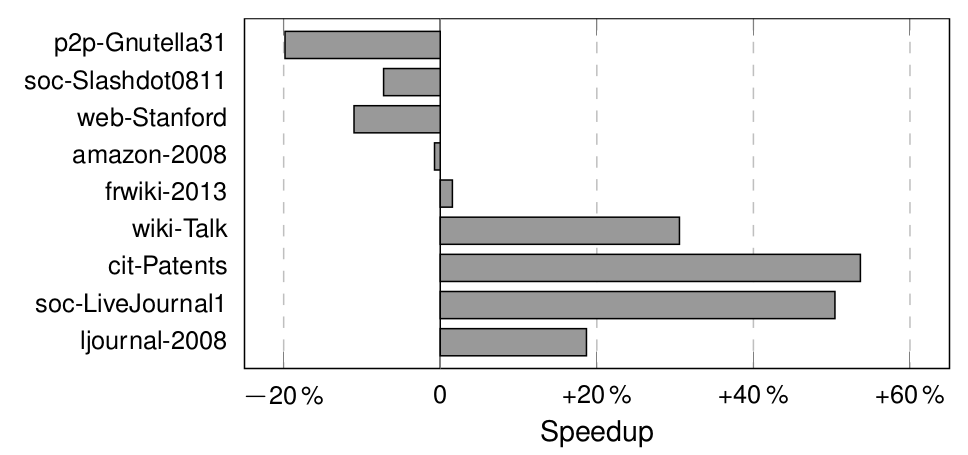
\includegraphics[width=0.8\linewidth]{pim_add.png}
  \caption{Performance improvement with an in-memory atomic addition operation
  used for the PageRank algorithm.}
\end{figure}

\chapter{Literature Survey}
\section{PIM Enabled Instruction}
For easier adoption of PIM, we desire little to no change in programmer's model.
Main memory products with integrated full-fledged processors with new
programming models may also not be available in the near future because of the
associated design complexity and changes required across the hardware/software
stack. Also, prior proposals do not utilize the benefits of on-chip caches and
virtual memory. This paper overcomes these challenges by extending the ISA of
the host processor with PIM-Enabled Instructions(PEIs)\cite{PEI_ISCA}, without chaning the
existing programming model. 


The paper proposes simple ISA extensions and the architectural support required
to integrate such simple operations into conventional systems.
The architecture proposes a restriction on the memory region accessible by
a single PIM operation is limited to a single last-level cache block. This
ensures the data can be accessed by the same vertical link and simplifies the
locality profiling.

\begin{figure}[h]
  \centering
  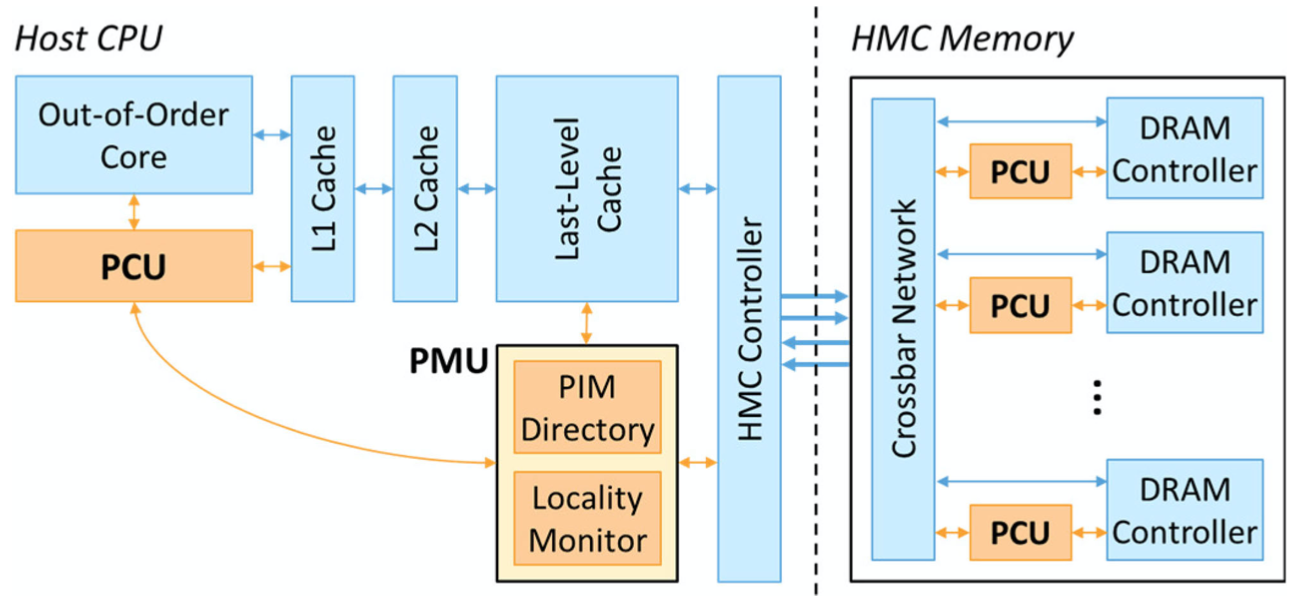
\includegraphics[width=0.8\linewidth]{PEI.png}
  \caption{Overview of the proposed architecture.}
\end{figure}

\subsection{PIM Compute Unit(PCU)}
PCU is a hardware unit that executes PEIs. All PCUs in the system have the same
computation logic so that any PEI can be executed by any PCU. In the proposed
architecture one PCU is placed besides every core in the host processor and one
PCU is placed in every vault. PCU has a SRAM based operand buffer to store
information of in-flight PEIs. 

\subsection{PIM Management Unit(PMU)}
The function of PMU is to 
\begin{itemize}
  \setlength\itemsep{0em}
    \item Ensure atomicity among different PEIs
    \item Maintain cache coherancy between memory and cache during PIM
      operation
    \item Profile data locality for locality aware execution
\end{itemize}

\subsubsection{PIM Directory}
PIM Directory ensures atmoicity among different in-flight PEIs. Atomicity
between a PEI and normal memory instruction is not maintained by PIM Directory.
This must be maintained by the programmer by using pfence. 
PIM Directory is a directly mapped, tag-less table indexed by XOR-folded addresses of 
target cache blocks. Each entry implements a reader-writer pair lock 


\subsubsection{Cache Coherancy Management}
Since the PEIs are resisted to a single last-level cache block, the cache
coherency problem is simplified. Whenever the PEI is executed on the host
processor the correspoinding last level block is flushed out and subsequent
blocks in L1 and L2 are back-invalidated. Thus ensuring neither the memory nor
the processor has a stale copy of data.

\subsubsection{Locality Monitor}
The key idea behind locality monitor is to decide whether to execute the PEI
locally on the host or remotely in the memory. Locality monitor is a taf array
with same number of sets/ways as that of the last-level cache. The key
difference between the locality monitor and the tag array fo the last-level
cache is that the formeris also updated when a PIM operation is issued to
memory. In our locality monitor, the data locality of a PEI can be
identified by checking to see if its target cache block address
hits in the locality monitor.

\subsection{PEI execution}
\subsubsection{Host-side PEI execution}
\begin{enumerate}
  \setlength\itemsep{0em}
  \item The out-of-order core writes the input operands to the memory-mapped
    registers of the PCU and issues the PEI
  \item PIM Directory then checks for atomicity and data locality - which
    results in high locality of data indicating host-side execution
  \item The PCU loads the block from cache and executes the instruction
  \item After execution the PCU writes back the output operands in the cache
    and notifies the PMU for completion
  \item The out-of-order core then reads the output operands using the
    memory-mapped registers of PCU.
\end{enumerate}

\begin{figure}[h]
  \centering
  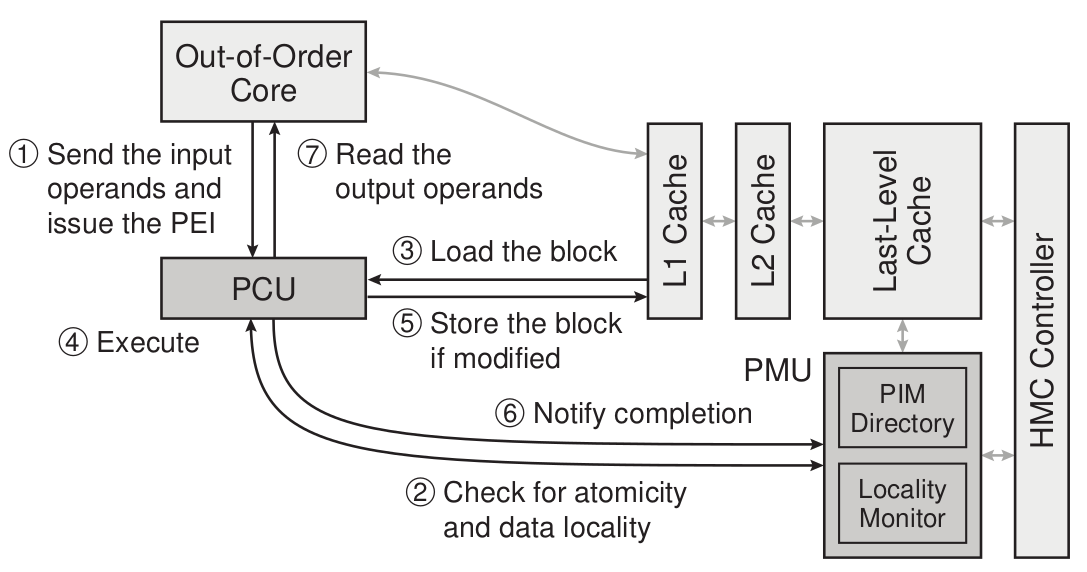
\includegraphics[width=0.8\linewidth]{host.png}
  \caption{Host-side PEI execution}
\end{figure}

\subsubsection{Memory-side PEI execution}
\begin{enumerate}
  \setlength\itemsep{0em}
  \item The out-of-order core writes the input operands to the memory-mapped
    registers of the PCU and issues the PEI
  \item PIM Directory then checks for atomicity and data locality - which
    results in low locality of data indicating memory-side execution
  \item The Last-level block in cache is flushed and the corresponding blocks
    in L1 and L2 are back-invalidated
  \item The host side PCU sends the input operands to the memory side PCU using
    the HMC controller
  \item The PCU executes the operation and sends back the output operands 
    indicating completion
  \item The out-of-order core then reads the output operands using the
    memory-mapped registers of PCU.
\end{enumerate}

\begin{figure}[h]
  \centering
  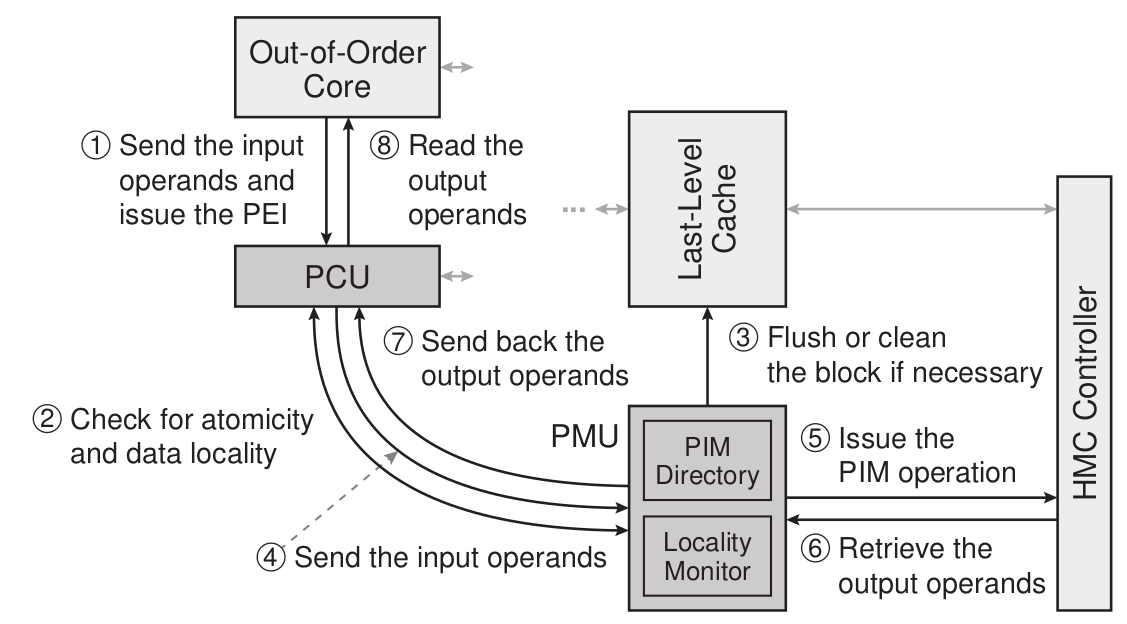
\includegraphics[width=0.8\linewidth]{memory.png}
  \caption{Memory-side PEI execution.}
\end{figure}



\subsection{Results}
\begin{itemize}
  \setlength\itemsep{0em}
  \item For large inputs, PIM-Only achieves 44\% speedup over Ideal-Host since using PIM 
    operations better utilizes the vertical DRAM bandwidth inside HMCs
  \item For small inputs, PIM-Only degrades average performance by 20\% because PIM 
    operations always access DRAM even though the data set comfortably fits in on-chip 
    caches
  \item Locality-Aware system provides the speedup of PIM-Only in workloads with large
inputs (47\% improvement over Host-Only) by offloading 79\% of PEIs to memory-side PCUs.
  \item Locality-Aware system provides the speedup of PIM-Only in workloads
    with small inputs (32\% improvement over Host-Only) by offloading 86\% of PEIs to 
    memory-side PCUs.
  \item Locality-Aware often outperforms both Host-Only and PIM-Only by simultaneously 
    utilizing host-side and memory-side PCUs for PEI execution
\end{itemize}
\begin{figure}[h]
  \centering
  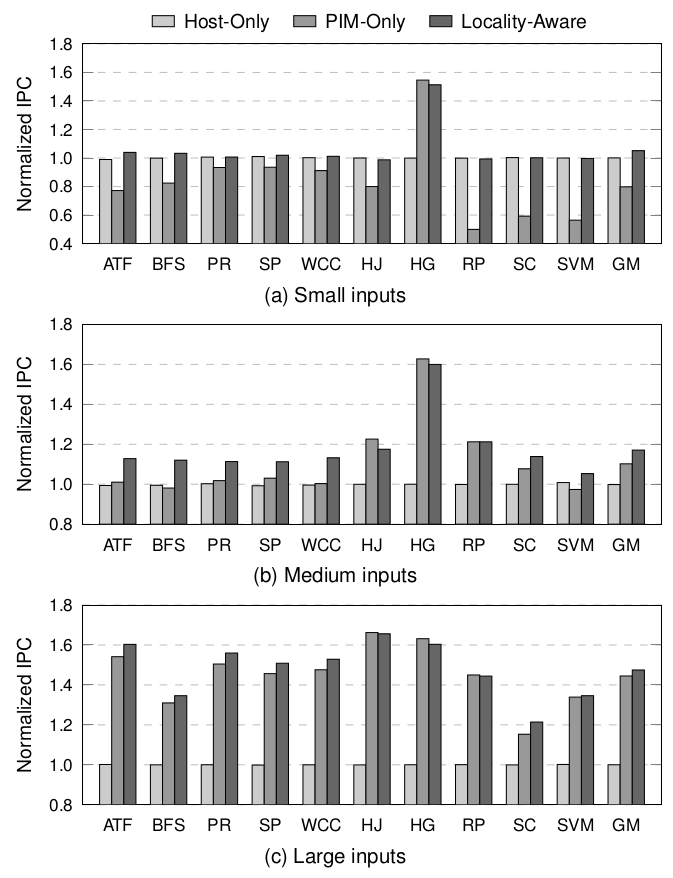
\includegraphics[width=0.7\linewidth]{results.png}
  \caption{Speedup comparison under different input sizes.}
\end{figure}

\subsection{Conclusion}
\begin{itemize}
  \setlength\itemsep{0em}
  \item PIM-enabled instructions (PEIs) is a practical model for processing-in-memory 
    and its hardware implementation, which is compatible with existing cache coherence 
    and virtual memory mechanisms
  \item PEIS have a last-level cache block restriction to ensure atomicity. 
  \item PEIs use data locality to decide the processing core.
\end{itemize}
 
\chapter{Future Work}
I plan to read the following conference papers -
\begin{itemize}
  \setlength\itemsep{0em}
  \item A. Devic  et al., "To PIM or not for emerging general purpose processing in
    DDR memory systems". In Proceedings of the 49th Annual International
    Symposium on Computer Architecture (ISCA '22). Association for Computing
    Machinery, New York, NY, USA, 231–244.
  \item K. Hsieh et al., "Transparent Offloading and Mapping (TOM): Enabling Programmer-Transparent Near-Data Processing in GPU Systems," 2016 ACM/IEEE 43rd Annual International Symposium on Computer Architecture (ISCA), 2016, pp. 204-216,
 
\end{itemize}

\bibliographystyle{ieeetr}
\bibliography{thesisTemplate}{}














\end{document}
